\documentclass[11pt,a4paper]{article}
\usepackage[english]{babel}
\selectlanguage{english}
\usepackage[T1]{fontenc}
\usepackage[utf8]{inputenc}
\usepackage[left=2.00cm, right=2.00cm, top=2.00cm, bottom=2.00cm]{geometry}
\usepackage{enumitem}
\usepackage{siunitx}
\usepackage{graphicx}
\usepackage{titling}
\usepackage{textcomp}
\usepackage{comment} 
\usepackage{multicol}
\usepackage{caption}
\usepackage{xcolor} 
\usepackage{booktabs}


\setlength{\droptitle}{-4\baselineskip} % Move the title up

\title{Structural Bioinformatics level III - Report of Project}
\author{
    \textsc{Tanguy Lallemand} \\[1ex] 
    \normalsize M2 Bioinformatics, NANTES \\ 
}
\date{\today}
\begin{document}
    \maketitle
    \section{Introduction}
    
    
    
    
    Structural protein modelling is a major challenge for bioinformatics. Indeed, many problems remain to model or predict structures of proteins. One approach to solve this type of problem is the use of protein blocks, which simplify modelling and prediction by simplifying a 3D structure into a 1D structure on which it is possible to apply proven algorithms such as sequence alignments. According to the authors, all conformations of 5 successive amino acid residues can be represented using one of the 16 protein blocks \cite{brevern_etchebest_hazout_2000}. Using this structural alphabet it is possible to approximate the local structure of a 3D protein structure. The use of this alphabet has a particular interest because the protein blocks are of size 5. This has several advantages, including being able to maintain local contacts within traditional structures such as $\beta$-sheets and $\alpha$-helices. Moreover, it is a good compromise between precision in 3D structure modelling and in prediction \cite{brevern_etchebest_hazout_2000}.\\
    From the primary sequence of a protein, it is possible to assign secondary structures for each amino acid as well as to obtain different information and in particular dihedral angles using tools such as \textbf{DSSP}. Indeed, the peptide skeleton contains three covalent bonds by amino acids, one of which is a flat bond. There are however, two simple links where rotation is possible. The rotation angles are called $\phi$ and $\psi$ respectively. These angles are partly constrained since some contacts of atoms too close are energetically unfavourable. These provide us informations on the position of amino acids in relation to each other and help to build peptide backbone. Thus a protein block according to this structural alphabet \cite{brevern_etchebest_hazout_2000} is composed of a succession of 8 dihedral angles allowing to represent the local pattern of the 5 amino acids concerned. 

    We will then try to study the characteristics of these protein blocks and more particularly block A. Different methods exist in data analysis and few of them can help to study backbone of protein block A. First of all, there are so-called factorial methods which are essentially linear and makes possible to reduce dimensions while seeking to lose as little information as possible. The most well known method is the \textbf{Principal Component Analysis} (PCA). This method makes it possible to project quantitative data and gathers an approach that is both geometric by representing the variables according to the directions of maximum inertia and statistical by looking for independent axes that explain the maximum variance of data.\\
    There are also classification methods that allow individuals to be grouped together following different criterais. There is in particular the mobile centre method (\textbf{k-means}) based on the \textbf{Forgy algorithm} \cite{macqueen1967}, but this method change only one vector at each adaptation cycle which makes this algorithm very slow. This method is still considered as reliable in literature and is still used \cite{bouvier_evrard-todeschi_girault_bertho_2009}. Another very known method is the \textbf{hierarchical ascending classification} (HAC) which does not require to know the number of classes \textit{a priori}.\\
    To finish, there is neural methods that are increasingly used. One of the best known methods is the \textbf{Kohonen Self Organizing Map} (SOM). This approach appears to be a generalisation of the \textbf{Forgy stochastic algorithm} \cite{macqueen1967}. K-means can be considered as a Kohonen algorithm with 0 neighbours. This unsupervised classification algorithm aims to group observations into classes but taking into account the topology of the observation space, including in this way, a notion of neighbourhood between classes. This approach has several advantages. First of all, it allows a non-linear projection of data. Moreover, its implementation is relatively simple and the cost in calculation is low compared to other methods. But also, the fact that no \textit{a priori} knowledge is necessary and results produced are relatively simple to interpret. This method is very common in literature and was used many times to solve similar problems \cite{bouvier_evrard-todeschi_girault_bertho_2009} \cite{schuchhardt_schneider_reichelt_schomburg_wrede_1996} \cite{brevern_etchebest_hazout_2000}.\\
    Thus, to solve the problem of this project which is to try to classify protein blocks A, it seems that a good approach would be to build a trained Kohonen map to be able to differentiate protein blocks A.
    
    
    
    \section{Methodology - Experimental Design}
    
    To begin, it is necessary to start by constructing a training data set containing all the dihedral angles of protein blocks A. This could have been built using the script \textbf{create\_protein\_blocks.sh} provided with the project but we use the data set provided. This one gathers the 8 dihedral angles of 68348 protein blocks A (PB a). These do not of course belong to the same proteins since this data set only contains protein blocks A coming from different proteins. \\
    The principle of this algorithm is as follows. First of all, the matrix gathering all the neurons is initialised with random data \cite{schuchhardt_schneider_reichelt_schomburg_wrede_1996}. This algorithm is iterative, which means it will read a given number of cycles the complete data set. Then, each value of the data set (here a protein block that is a vector of 8 angles) is compared to values of each neurons ( neuron and associated weight is called a class of object in machine learning terminology). In the case of this project, the comparison between vector from data set and each class of object is made using the RMSD calculation which determines the structural proximity of two structures.
    RMSD is calculated using equation \ref{rmsd}.
    \begin{equation}
    \label{rmsd}
        \mathrm{RMSD}(\mathbf{v}, \mathbf{w}) & = \sqrt{\frac{1}{n}\sum_{i=1}^{n} \|v_i - w_i\|^2} \\
        & = \sqrt{\frac{1}{n}\sum_{i=1}^{n} 
              (({v_i}_x - {w_i}_x)^2 + ({v_i}_y - {w_i}_y)^2 + ({v_i}_z - {w_i}_z)^2})
    \end{equation}
    
    The neuron with the closest RMSD is then determined as the winning neuron. This neuron is brought closer to the value that has just been assigned to it. This change is weighted by the learning rate. This update of neuron is calculated using equation \ref{update_neuron} as follows:
    \begin{equation}
        \label{update_neuron}
        w^{k}(t+1) = w^{k}(t) + \left [ v - w^{k}(t) \right ]\eta e^{-\frac{1}{2r^{2}}(r^{k} - r^{next})^{2}}
    \end{equation}
    With $w^{k}(t+1)$ as the new value of the neuron, $w^{k}(t)$ the actual value of the neuron, $\eta$, the learning rate and \textit{r} the learning radius.\\
    Neighbouring classes also receive some of this information to a lesser extent. The transmission of information is more or less strong depending on the distance from the neuron to the winning neuron. The further away the class is, the less information it will receive. This is possible by weighting the learning radius (\textit{r} in the equation of update of each neuron).
    This algorithm is iterative, so the data set is used several times. Convergence is allowed by the fact that the learning rate  and the learning radius are updated at each iteration using (equation \ref{learning_rate} and \ref{learning_radius}). These rates updates are made by the following formulas:
    \begin{equation}
        \label{learning_rate}
       \eta (t) = \frac{\eta _{0}}{1+\frac{i}{\tau }}
    \end{equation}
    
    \begin{equation}
        \label{learning_radius}
       r(t) = \frac{r_{0}}{1+\frac{i}{\tau }}
    \end{equation}
    
    Hence, it is possible to impact the algorithm in different ways. In addition to the fact that we can determine the number of neurons, it is also possible to impact it through the topology of the map, which in our case will not have to be done. Moreover, it is possible to choose the initial learning rate as well as the learning radius. To finish, the number of iterations of the algorithm remains to be determined.
    
    For this project, the Kohonen algorithm was implemented using R. The code used is provided with the project. Code was splited into two files, one storing functions used and the other managing function calls and the global algorithm. Please notice that this script can receive some parameters. To have list of possible parameters please call: \textbf{./self\_organizing\_map.R --help}. Results are outputed as a multiple graph gathering for each neuron the different angles assigned to them.\\
    The algorithm was executed using different parameters that can be passed as parameters at the script's launch. Indeed, it is known that this type of method requires fine tuning in order to produce good results. The different results will be discussed in the following section.
    
    
    \section{Results}
    
    
    Thus the algorithm was tested with first of all relatively median parameters namely: a learning rate of 0.75, a learning radius of 2 and one iteration. The results produced are shown in the figure \ref{fig:mutliple_graph_learn_rate_0_75_2_1}. Moreover, details of each dihedral angles are provided in table \ref{theorical}. Graph shows that algorithm has converged and each neurons represent well PB a. This can be confirmed by the table \ref{theorical} that show the detail of each angle in the theorical model and in the case of the neuron in the upper left corner. We can notice that with those parameters one iteration is enough, in fact same calculation were run on three iterations and results produced are similar (graph not provided). \\
    To follow, the following parameters: learning rate of 0.1, learning radius of 0.5 and 1 iterations have been used, the results are provided in the graph \ref{fig:mutliple_graph_learn_rate_0_1_0_5_1}. With these parameters, neurons doe not seem to have learned enough. Indeed, only the 4 neurons at the bottom right corner have integrated the information and represent right backbone of PB a. One more graph has been built using learning rate of 0.75, learning radius of 0.5 and 3 iterations and produce similar results. Thus, the number of iterations and the learning rate do not seem to have played a significant role. Indeed, the 4 neurons have learned the information well but not the whole topological map. It would therefore seem that it is the learning radius that is too small and that would not allow the information to be transmitted even with a higher number of iterations.\\

    To finish we try to use more neurons to see impact on result. Script was implemented with maximum of modularity and change number of neurons is simple. We try with 36 neurons, computing time increase enormously. Results are provided in graph \ref{mutliple_graph_36_neurons_learn_rate_1_1_1}. Hence, by increasing number of neurons, even if with a good learning rate and radius algorithm did not totally converge after one iteration. In fact, the neuron in the upper left corner does not store right backbone. This suggest that precedent hypothesis are quite good and learn radieux need to be balanced with size of map.
    
    
    \section{Discussion}
    
    About the implementation of the algorithm, it seems sufficient, the calculation time is quite long, perhaps optimizations can be made. The management of the algorithm configuration by passing by parameters the values allows to launch and quickly the calculations in command, and allowing to parallelize the calculation launches and run multiple test of parameters at the same time. \\
    
    The difference between vector of the data set and the object classes is determined by the calculation of the RMSD, an approach that has already been done in literature \cite{brevern_etchebest_hazout_2000} \cite{schuchhardt_schneider_reichelt_schomburg_wrede_1996} and seems to be reliable. 
    Results seems to be relatively good using a learning rate of 0.75, learning radius of 2 and 1 or 3 iterations. In fact, when details of each neuron content is compared to theorical data for PB A gathered from literature \cite{article}, neurons contains dihedral angles pretty close. Content from one neuron and theorical data are provided in table \ref{theorical}. So the Kohonen algorithm seems to produce good results on this training data set for PB a. Moreover, the fact that with appropriate parameters all neurons have a similar backbone is logical since we were trying to make an Self Organising Map on a data set containing only protein block A. \\
    
    
    All these results suggest that the learning radius seems to be the parameter that has the greatest impact on the results since it allow to modulate how the information is passed to neighbouring classes. Thus a too low radius will not allow a convergence of the algorithm in a reasonable number of iterations. Nevertheless, we can hypothesize that with a large number of iterations the information would eventually reach all neurons. Hence, this parameter must be considered at the same time as the number of iterations and a balance must be found between them.  However, a too large learning radius can be improper if the SOM is used to classify different protein blocks, indeed in this case the goal is not to obtain the same backbone on the whole map. To finish, by working on a map with only 16 neurons, we can wonder if the impact of the learning radius has a biased impact due to the small size of our neuron matrix. In literature, we found some papers where number of neurons is more around 100 \cite{schuchhardt_schneider_reichelt_schomburg_wrede_1996} even if some papers suggest that smaller SOM can produce more reliable clustering \cite{bouvier_evrard-todeschi_girault_bertho_2009}.\\
    The learning rate does not seem to have a strong impact on the results of the algorithm, we can wonder if this is not due to the fact that first of all, we use a training data set with "perfect" data but also that it is of sufficient size to make learning good even with a reduced rate. A good learning rate can nevertheless save computing time by reducing the number of iterations required for convergence.\\

    In order to improve this project several additions could be possible. We can see that after a certain number of iterations and depending on the learning radius, the algorithm may have converged well before the end of the learning radius. It might therefore be interesting to implement a way to cut the algorithm if it has converged in order to save computing time.\\
    From a more distant perspective, it may be interesting to look at potential alternatives that may be more appropriate in some cases. And in particular some known alternatives like following methods. Time Adaptive Self-Organizing Map (TASOM) \cite{1187438} which is an algorithm that allow to use adaptive learning rates allowing to avoid a step of optimization of parameters. There is also Growing Self-Organizing Map (GSOM), a method that avoid problems about size of Kohonen map by determining herself size of map. Using those alternatives  can help to avoid a part of steps of configuration allowing to work with best parameters.\\

    To conclude, we have therefore succeeded in developing an R algorithm that allows for a non supervised classification using the Kohonen algorithm. The output allows to visualise all the dihedral angles of each neuron. With the right parameters each neuron provides the similar vector of dihedral angles that appear to be dihedral angles of protein block A's backbone appearing in \cite{brevern_etchebest_hazout_2000}. Unfortunately, the fine tuning of this algorithm remains difficult and time consuming, interesting alternatives such as TASOM or GSOM could avoid these tweaking phases.
    
    
    %choix du style de la biblio
    \bibliographystyle{ieeetr}
    %inclusion de la biblio
    \bibliography{biblio.bib}
    
    \section{Annexes}
    \begin{figure}[h!]
        \centering
        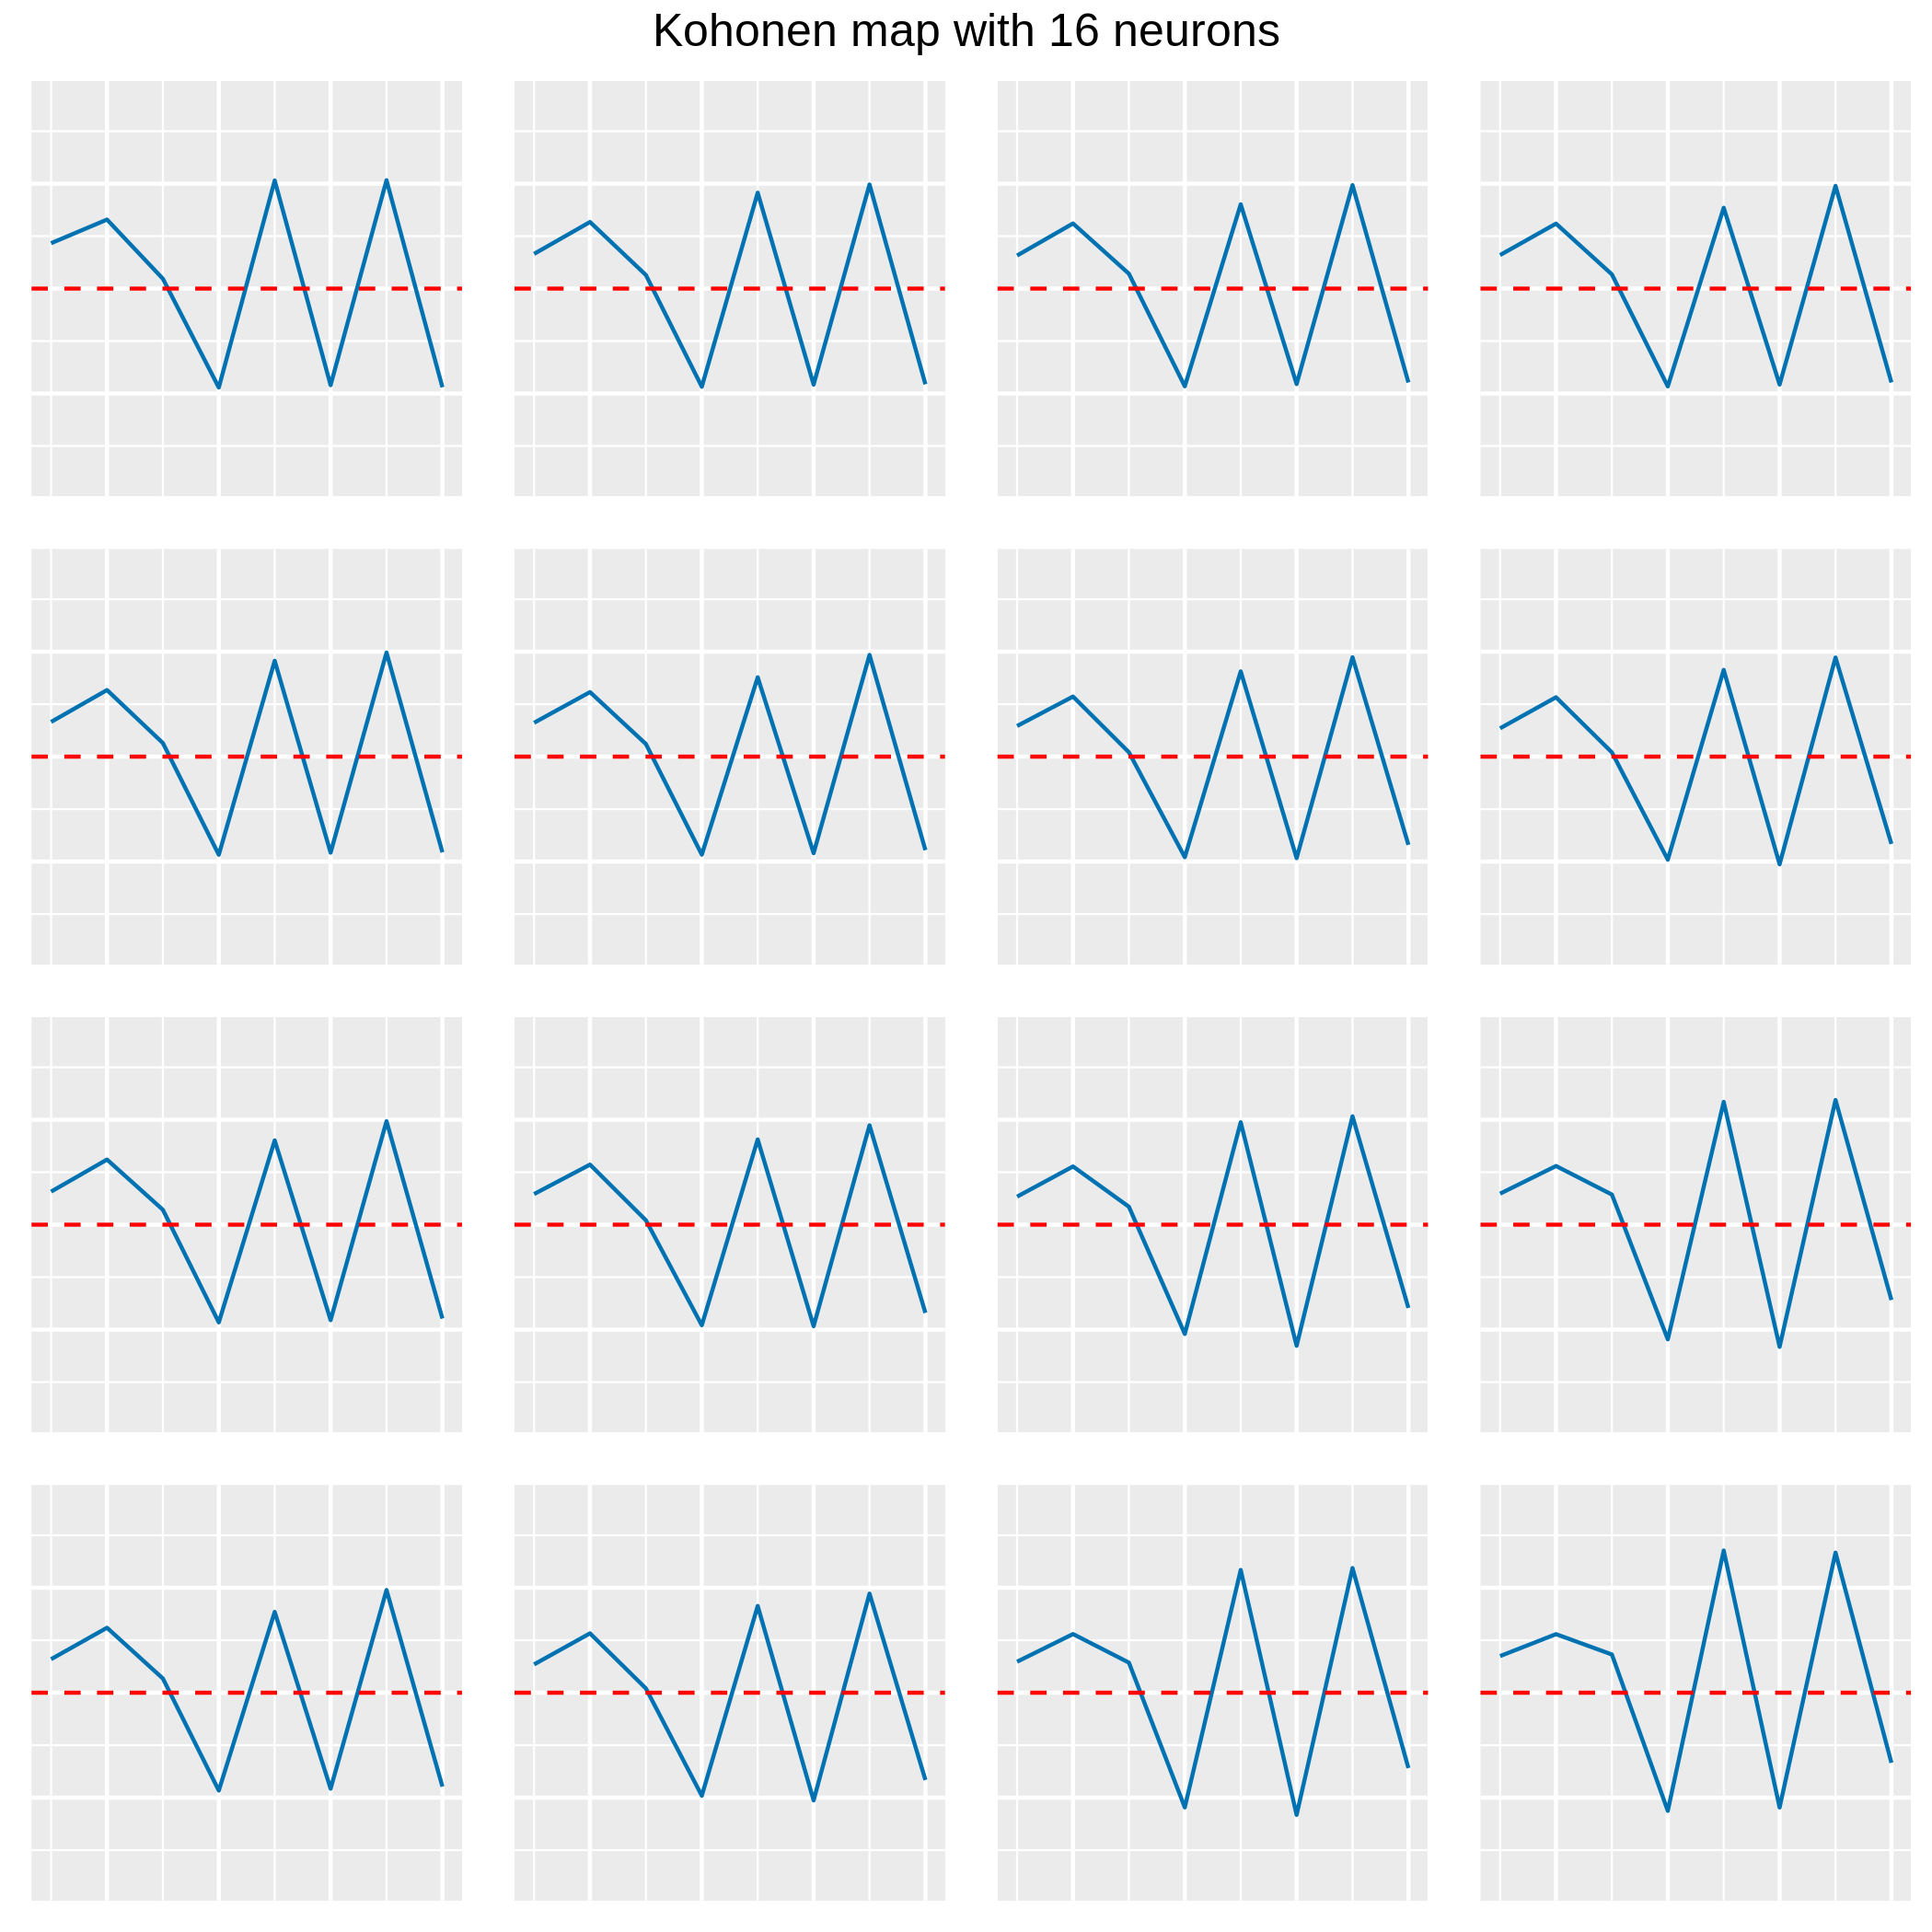
\includegraphics[height=10cm]{img/mutliple_graph_learn_rate_0_75_2_1.png}
        \caption{Kohonen map with 16 neurons computed using following parameters: learning rate of 0.75, learning radius of 2 and 1 iterations}
        \label{fig:mutliple_graph_learn_rate_0_75_2_1}
    \end{figure}
    \begin{figure}[h!]
        \centering
        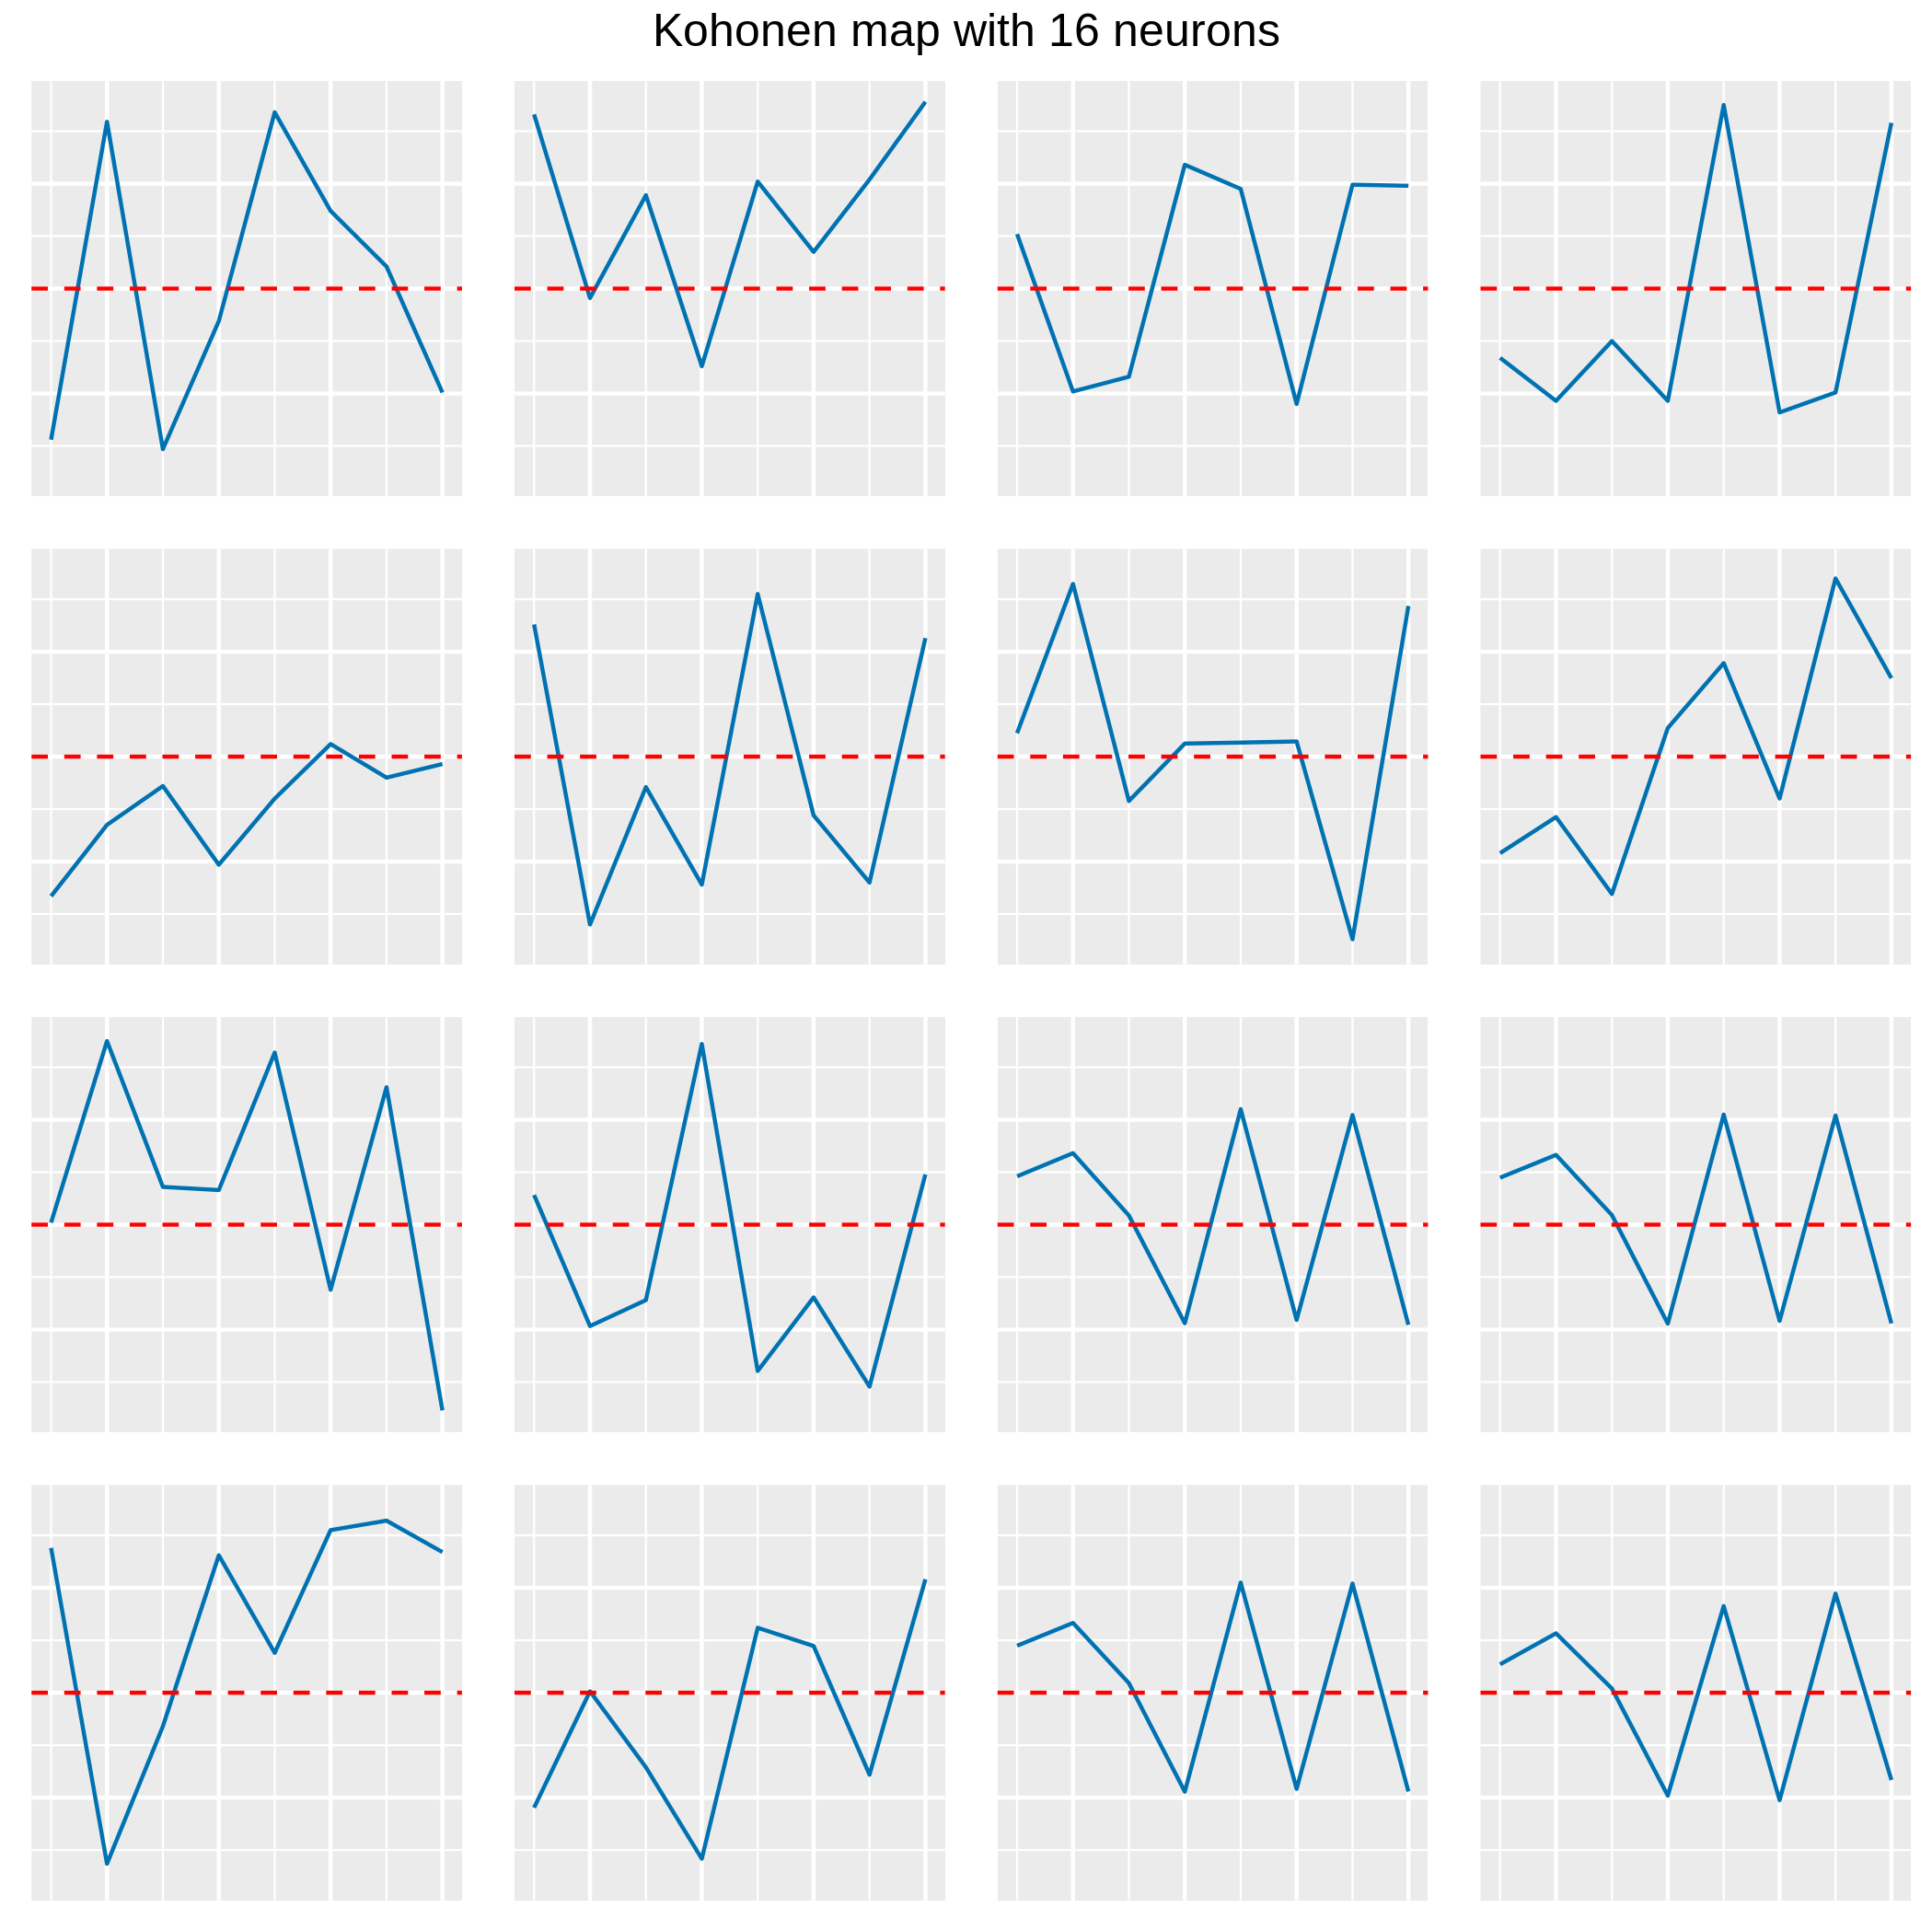
\includegraphics[height=10cm]{img/mutliple_graph_learn_rate_0_1_0_5_1.png}
        \caption{Kohonen map with 16 neurons computed using following parameters: learning rate of 0.1, learning radius of 0.5 and 1 iterations}
        \label{fig:mutliple_graph_learn_rate_0_1_0_5_1}
    \end{figure}
    \begin{figure}[h!]
        \centering
        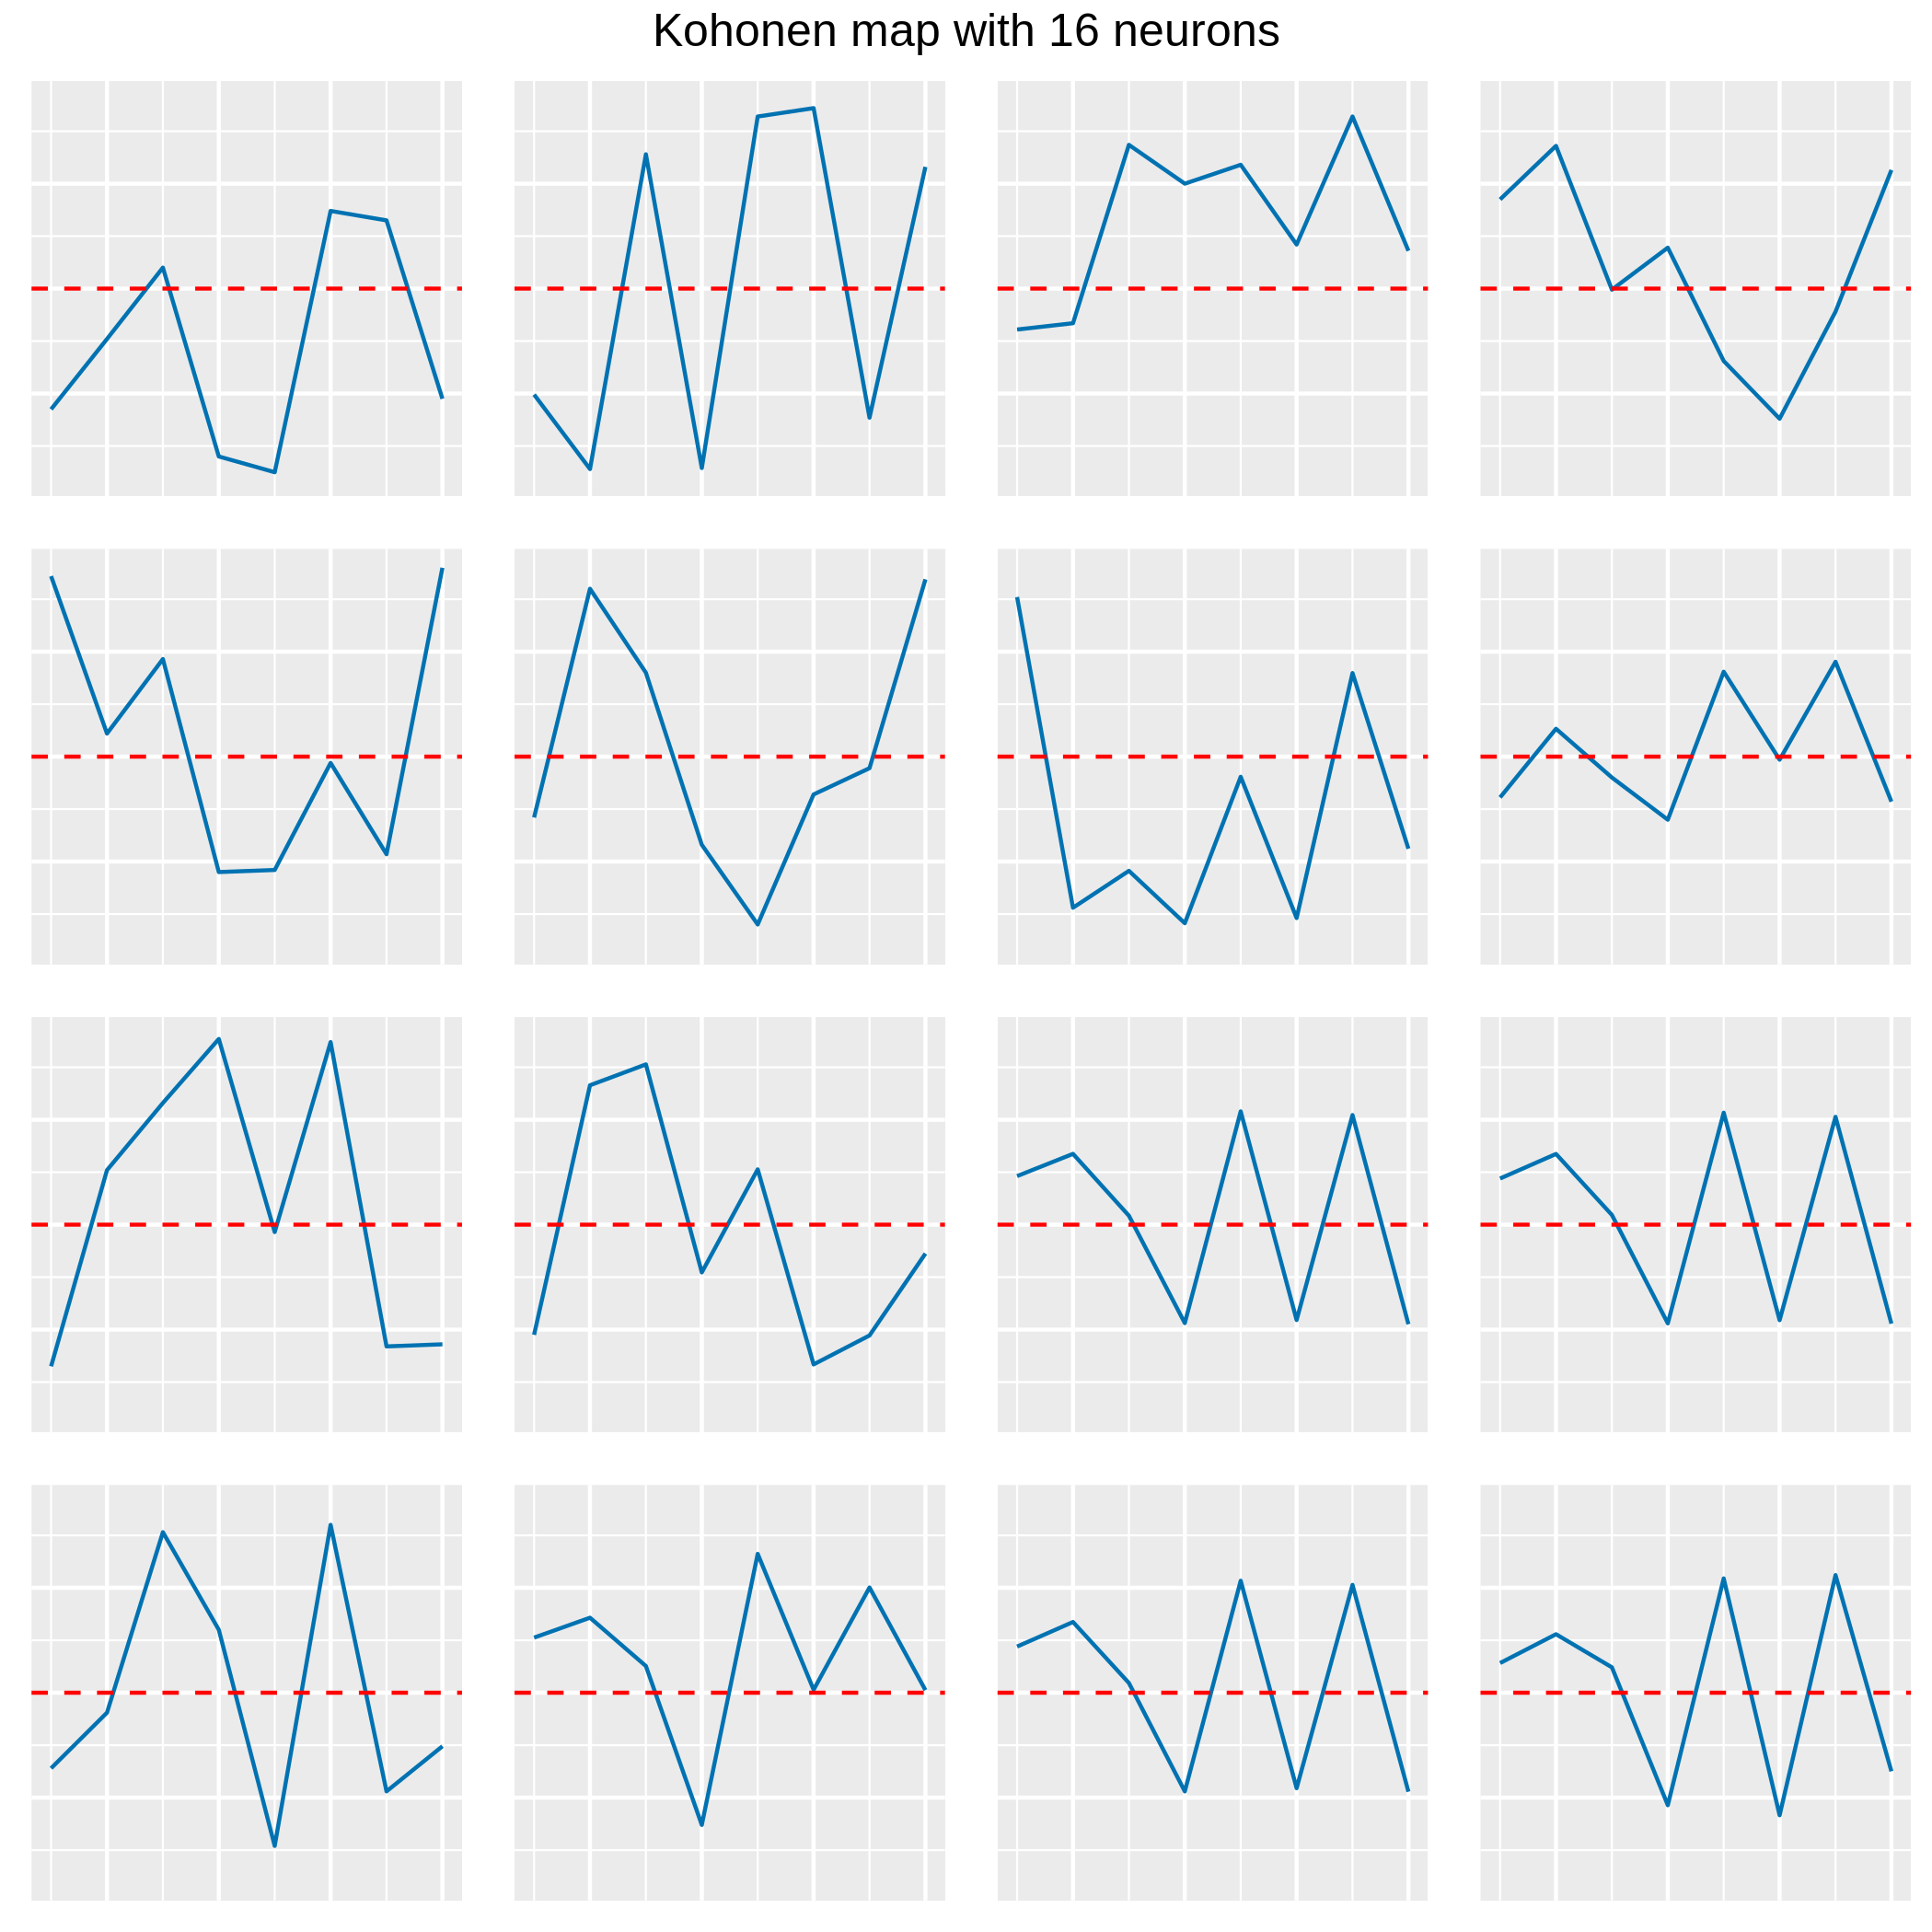
\includegraphics[height=7cm]{img/mutliple_graph_learn_rate_0_75_0_5_3.png}
        \caption{Kohonen map with 16 neurons computed using following parameters: learning rate of 0.75, learning radius of 0.5 and 3 iterations}
        \label{fig:mutliple_graph_learn_rate_0_75_0_5_3}
    \end{figure}
    \begin{figure}[h!]
        \centering
        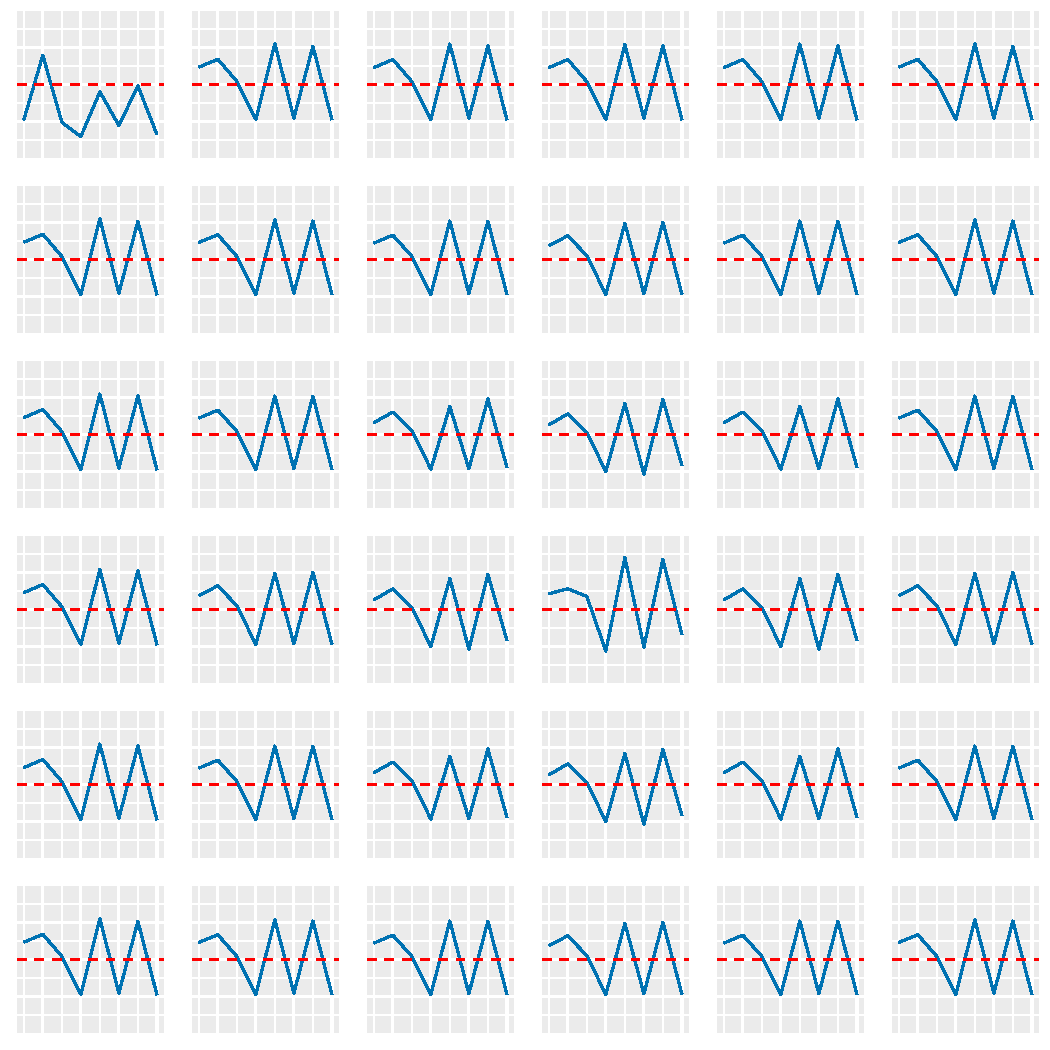
\includegraphics[height=7cm]{img/mutliple_graph_36_neurons_learn_rate_1_1_1.pdf}
        \caption{Kohonen map with 36 neurons computed using following parameters: learning rate of 1, learning radius of 1 and 1 iterations}
        \label{fig:mutliple_graph_36_neurons_learn_rate_1_1_1}
    \end{figure}
    
    \begin{table}[h!]
        \centering
        \begin{tabular}{|l|l|l|l|l|l|l|l|l|}
        \hline
        Dihedral angle & $\psi_{i-2}$ & $\phi_{i-1}$ & $\psi_{i-1}$ & $\phi_{i}$ & $\psi_{i}$ & $\phi_{i+1}$ & $\psi_{i+1}$ &  $\phi_{i+2}$ \\ \hline
        Theorical result & 41.14 & 75.53 & 13.92 & -99.80 & 131.88 & -96.27 & 122.08 & -99.68 \\ \hline
        Neuron result & 44.22 & 66.69 & 9.13 & -94.19 & 105.31 & -91.19 & 103.26 & -94.19  \\ \hline
        \end{tabular}
        \caption{Vectors of dihedral angles for PB a from literature and from one neuron in a Kohonen map computed with following parameters: learning rate of 0.75, learning radius of 2 and 3 iterations }
        \label{theorical}
    \end{table}
    

\end{document}
